\documentclass[10pt,a4paper]{article}
\usepackage[utf8]{inputenc}

% Define the page margin
\usepackage[margin=3cm]{geometry}

% Better typography (font rendering)
\usepackage{microtype}

% Math environments and macros
\usepackage{amsmath}
\usepackage{amsfonts}
\usepackage{amssymb}
\usepackage{amsthm}

% Define \includegraphics to include graphics
\usepackage{graphicx}

% Draw graphics from a text description
\usepackage{tikz}

% Syntax highlighting
\usepackage{minted}

% Set global minted options
\setminted{linenos, autogobble, frame=lines, framesep=2mm}

% Import the comment environment for orgtbl-mode
\usepackage{comment}

% Do not indent paragraphs
\usepackage{parskip}

\title{Randomized Algorithms, Sheet 9}
\author{Marten Lienen (03670270)}

\begin{document}

\maketitle

\section*{Exercise 9.1}

The same algorithm that we developed in class can be used here as well to show that there is always a marriage without strong instabilities.
If there were a strong instability in the end, the man would have proposed to his preferred woman before proposing to his current partner and the woman would have accepted him over her current partner respectively not let him go for her current partner.
The introduction of indifference does not change that.

On the other hand there are scenarios where a weak instability is unavoidable.
Let for example be $m_{1}, m_{2}$ two men and $w_{1}, w_{2}$ two women where then men are indifferent between the women but but women prefer $m_{1}$ over $m_{2}$.
Now in either of the two possible marriages $\{ (m_{1}, w_{1}), (m_{2}, w_{2}) \}$ and $\{ (m_{1}, w_{2}), (m_{2}, w_{1}) \}$ the woman that is not married to $m_{1}$ will prefer him over her current partner while $m_{1}$ is indifferent between them.

\section*{Exercise 9.2}

Let $X$ be the total number of heads.
Then $X$ is binomially distributed with success probability $\frac{1}{2}$, $100$ tries, expected value $E[X] = \frac{1}{2}100 = 50$ and variance $Var[X] = 100 \cdot \frac{1}{2} \cdot \frac{1}{2} = 25$.
Now we will bound the probability of obtaining $n$ or more heads in the three different ways and start out with Markov's inequality.

\begin{equation*}
  P[X \ge n] \le \frac{E[X]}{n} = \frac{50}{n}
\end{equation*}

Next we use Chebyshev's inequality.

\begin{align*}
  P[X \ge n] & = P[X - E[X] \ge n - E[X]]\\
             & \le P[|X - E[X]| \ge n - E[X]]\\
             & \le \frac{Var[X]}{(n - E[X])^{2}} = \frac{25}{(n - 50)^{2}}
\end{align*}

Finally we obtain a bound using Chernoff bounds.

\begin{align*}
  P[X \ge n] & = P[X \ge \frac{n}{E[X]}E[X]]\\
             & = P[X \ge \left( 1 + \frac{n - E[X]}{E[X]} \right)E[X]]\\
             & \le \left[ \frac{\exp\left( \frac{n - E[X]}{E[X]} \right)}{\left( \frac{n}{E[X]} \right)^{\frac{n}{E[X]}}} \right]^{E[X]}\\
             & = \left[ \frac{\exp\left( \frac{n - 50}{50} \right)}{\left( \frac{n}{50} \right)^{\frac{n}{50}}} \right]^{50}\\
             & = \frac{\exp\left( \frac{n}{50} - 1 \right)^{50}}{\left( \frac{n}{50} \right)^{n}}\\
             & = 50^{n} \frac{\exp\left( n - 50 \right)}{n^{n}}
\end{align*}

% BEGIN RECEIVE ORGTBL exercise-9-2
\begin{tabular}{lll}
Method & $n = 55$ & $n = 60$\\
\hline
Markov's inequality & $\frac{10}{11} \approx 0.91$ & $\frac{5}{6} \approx 0.83$\\
Chebyshev's inequality & $1$ & $\frac{1}{4} = 0.25$\\
Chernoff bound & $\approx 0.76$ & $\approx 0.39$\\
\end{tabular}
% END RECEIVE ORGTBL exercise-9-2
\begin{comment}
#+ORGTBL: SEND exercise-9-2 orgtbl-to-latex :splice nil :skip 0 :raw t
| Method                 | $n = 55$                     | $n = 60$                   |
|------------------------+------------------------------+----------------------------|
| Markov's inequality    | $\frac{10}{11} \approx 0.91$ | $\frac{5}{6} \approx 0.83$ |
| Chebyshev's inequality | $1$                          | $\frac{1}{4} = 0.25$       |
| Chernoff bound         | $\approx 0.76$               | $\approx 0.39$             |
\end{comment}

\section*{Exercise 9.3}

Unfortunately I do not understand the hint/part about representing the sum as a sum of indenpendent Poisson variables.
Instead I will just try to derive a Chernoff bound directly.

Let $t \in \mathbb{R}$ such that $\log(t) < 2 \Leftrightarrow t < e^{2}$.
\begin{align*}
  P[X > (1 + \epsilon)2n] & = P\left[ \exp(tX) > \exp(t(1 + \epsilon)2n) \right]\\
                          & = P\left[ \exp(tX) > \exp(t(1 + \epsilon)2n) \right]\\
                          & < \frac{E[\exp(tX)]}{\exp(t(1 + \epsilon)2n)}\\
                          & = \frac{E[\exp(t \sum_{i} X_{i})]}{\exp(t(1 + \epsilon)2n)}\\
                          & = \frac{\prod_{i} E[\exp(tX_{i})]}{\exp(t(1 + \epsilon)2n)}\\
                          & = \frac{\prod_{i} \sum_{k = 1}^{\infty} \exp(kt) \cdot \left( \frac{1}{2} \right)^{k}}{\exp(t(1 + \epsilon)2n)}\\
                          & = \frac{\prod_{i} \sum_{k = 1}^{\infty} \left( \frac{\exp(t)}{2} \right)^{k}}{\exp(t(1 + \epsilon)2n)}\\
                          & = \frac{\prod_{i} \frac{1}{1 - \frac{\exp(t)}{2}} - 1}{\exp(t(1 + \epsilon)2n)}\\
                          & = \frac{\prod_{i} \frac{2}{2 - \exp(t)} - 1}{\exp(t(1 + \epsilon)2n)}\\
                          & = \frac{\prod_{i} \frac{\exp(t)}{2 - \exp(t)}}{\exp(t(1 + \epsilon)2n)}\\
                          & = \frac{\frac{\exp(tn)}{(2 - \exp(t))^{n}}}{\exp(t(1 + \epsilon)2n)}\\
                          & = \frac{1}{(2 - \exp(t))^{n} \cdot \exp\left( (2(1 + \epsilon) - 1)tn \right)}\\
                          & = \frac{1}{(2 - \exp(t))^{n} \cdot \exp\left( (2\epsilon + 1)tn \right)}
\end{align*}

In the next step we minimize the upper bound over $t$.
The bound is minimized when the denominator is maximized, so we will look for a maximum of the denominator.
Its derivative with respect to $t$ is
\begin{equation*}
  -n\exp(t)(2 - \exp(t))^{n - 1} \cdot \exp((2\epsilon + 1)tn) + (2 - \exp(t))^{n} \cdot (2\epsilon + 1)n \exp((2\epsilon + 1)tn)
\end{equation*}
which can be simplified to
\begin{equation*}
  2n\left( (2\epsilon + 1) - (\epsilon + 1)\exp(t) \right) (2 - \exp(t))^{n - 1} \exp((2\epsilon + 1)tn)
\end{equation*}

The roots of the derivative are at $t$ where any of the factors is $0$.
This is either
\begin{equation*}
  2 - \exp(t) = 0 \Leftrightarrow t = \log(2)
\end{equation*}
or
\begin{equation*}
  (2\epsilon + 1) - (\epsilon + 1)\exp(t) = 0 \Leftrightarrow (2\epsilon + 1) = (\epsilon + 1)\exp(t) \Leftrightarrow t = \log\left( \frac{2\epsilon + 1}{\epsilon + 1} \right)
\end{equation*}
The first root can be excluded because first we required $t < \log(2)$ and secondly we would have to divide by zero in the upper bound.
The other root is however a legal value as $\log\left( \frac{2\epsilon + 1}{\epsilon + 1} \right) < \log(2)\ \forall \epsilon > 0$ and it has to be a maximum by the following argument.
The original bound that we computed is always positive since it is equal to a fraction that is obviously always positive because it consists of a fraction of exponential functions.
Since the denominator evaluates to $0$ for $t = \log(2)$, it has to have a minimum at $\log(2)$ for if there were another smaller point in a neighbourhood around $\log(2)$, if would have to be negative, which is not possible.
Now we know of another extremum at $\log\left( \frac{2\epsilon + 1}{\epsilon + 1} \right)$ which has a strictly positive distance to $\log(2)$ for all $\epsilon$.
Since the derivative evaluates to something non-zero between these, this second extremum has to be a local maximum.
Checking the limit towards $-\infty$ results in $1$, which makes the local maximum a global one.
Finally we get the bound

\begin{align*}
  P[X > (1 + \epsilon)2n] & < \frac{1}{\left(2 - \frac{2\epsilon + 1}{\epsilon + 1} \right)^{n} \exp\left( (2\epsilon + 1)n\log\left( \frac{2\epsilon + 1}{\epsilon + 1} \right) \right)}\\
                          & = \frac{1}{\left(\frac{1}{\epsilon + 1} \right)^{n}\left( \frac{2\epsilon + 1}{\epsilon + 1} \right)^{(2\epsilon + 1)n}}\\
                          & = \frac{(\epsilon + 1)^{(2\epsilon + 2)n}}{(2\epsilon + 1)^{(2\epsilon + 1)n}}
\end{align*}

\section*{Exercise 9.4}

\begin{proof}
  If $\delta = 1$, the upper bound evaluates to $1$ (if we assume $0^{0} = 1$) which always holds.
  So for the rest of this proof we assume $0 < \delta < 1$.

  Let $t \in \mathbb{R}_{\ge 0}$.
  \begin{align*}
    P[X \le (1 - \delta)\mu] & = P[\exp(tX) \le \exp(t(1 - \delta)\mu)]\\
                             & \le \frac{E[\exp(tX)]}{\exp(t(1 - \delta)\mu)}\\
                             & = \frac{E[\exp(\sum_{i} tX_{i})]}{\exp(t(1 - \delta)\mu)}\\
                             & = \frac{E[\prod_{i} \exp(tX_{i})]}{\exp(t(1 - \delta)\mu)}\\
                             & = \frac{\prod_{i} E[\exp(tX_{i})]}{\exp(t(1 - \delta)\mu)} \qquad \textit{because the $X_{i}$ are independent}\\
                             & = \frac{\prod_{i} \left( p_{i}\exp(t) + (1 - p_{i}) \exp(0) \right)}{\exp(t(1 - \delta)\mu)}\\
                             & = \frac{\prod_{i} \left( 1 + p_{i}\left( \exp(t) - 1\right) \right)}{\exp(t(1 - \delta)\mu)}\\
                             & = \frac{\prod_{i} \exp\left( p_{i}\left( \exp(t) - 1\right) \right)}{\exp(t(1 - \delta)\mu)} \qquad \textit{because $1 + x \le \exp(x)$}\\
                             & = \frac{\exp\left( \sum_{i} p_{i}\left( \exp(t) - 1\right) \right)}{\exp(t(1 - \delta)\mu)}\\
                             & = \frac{\exp\left( \left( \exp(t) - 1 \right)\mu \right)}{\exp(t(1 - \delta)\mu)}
  \end{align*}

  Since the previous inequality is true for any such $t$ we can just plug in $t = \log(1 - \delta)$.
  \begin{align*}
    P[X \le (1 - \delta)\mu] & \le \frac{\exp\left( \left( \exp(\log(1 - \delta)) - 1 \right)\mu \right)}{\exp(\log(1 - \delta)(1 - \delta)\mu)}\\
                             & = \frac{\exp\left( -\delta \mu \right)}{(1 - \delta)^{(1 - \delta)\mu}}\\
                             & = \left( \frac{\exp\left( -\delta \right)}{(1 - \delta)^{1 - \delta}} \right)^{\mu}
  \end{align*}

  It is left to show that
  \begin{align*}
    \left( \frac{\exp\left( -\delta \right)}{(1 - \delta)^{1 - \delta}} \right)^{\mu} \le \left( \frac{e^{\delta}}{(1 + \delta)^{1 + \delta}} \right)^{\mu} \Leftrightarrow &\quad \frac{e^{\delta}}{(1 + \delta)^{1 + \delta}} - \frac{e^{-\delta}}{(1 - \delta)^{1 - \delta}} \ge 0\\
    \Leftrightarrow &\quad e^{\delta}(1 - \delta)^{1 - \delta} - e^{-\delta}(1 + \delta)^{1 + \delta} \ge 0\\
    \Leftrightarrow &\quad e^{\delta + (1 - \delta)\log(1 - \delta)} - e^{-\delta + (1 + \delta)\log(1 + \delta)} \ge 0\\
    \Leftrightarrow &\quad \frac{e^{\delta + (1 - \delta)\log(1 - \delta)}}{e^{-\delta + (1 + \delta)\log(1 + \delta)}} \ge 1\\
    \Leftrightarrow &\quad e^{\delta + (1 - \delta)\log(1 - \delta) - (-\delta + (1 + \delta)\log(1 + \delta))} \ge 1\\
    \Leftrightarrow &\quad 2\delta + (1 - \delta)\log(1 - \delta) - (1 + \delta)\log(1 + \delta) \ge 0\\
    \Leftrightarrow &\quad 2\delta + \log\left( \left( 1 - \delta \right)^{1 - \delta} \right) - \log\left( \left( 1 + \delta \right)^{1 + \delta} \right) \ge 0\\
    \Leftrightarrow &\quad 2\delta + \log\left( \frac{\left( 1 - \delta \right)^{1 - \delta}}{\left( 1 + \delta \right)^{1 + \delta}} \right) \ge 0\\
    \Leftrightarrow &\quad \log\left( \frac{\left( 1 - \delta \right)^{1 - \delta}}{\left( 1 + \delta \right)^{1 + \delta}} \right) \ge -2\delta\\
    \Leftrightarrow &\quad \frac{1}{2\delta}\log\left( \frac{\left( 1 - \delta \right)^{1 - \delta}}{\left( 1 + \delta \right)^{1 + \delta}} \right) \ge -1\\
    \Leftrightarrow &\quad \log\left( \left(\frac{\left( 1 - \delta \right)^{1 - \delta}}{\left( 1 + \delta \right)^{1 + \delta}}\right)^{\frac{1}{2\delta}} \right) \ge -1\\
    \Leftrightarrow &\quad \left(\frac{\left( 1 - \delta \right)^{1 - \delta}}{\left( 1 + \delta \right)^{1 + \delta}}\right)^{\frac{1}{2\delta}} \ge \frac{1}{e}\\
  \end{align*}

  The $\lim_{\delta \rightarrow 0}$ of the left hand side is $1$ which is greater than $\frac{1}{e}$, so this inequality holds if the derivative of the left hand side is $\ge 0$ for $0 < \delta < 1$.
  A quick check with wolframalpha shows that this is indeed true.

  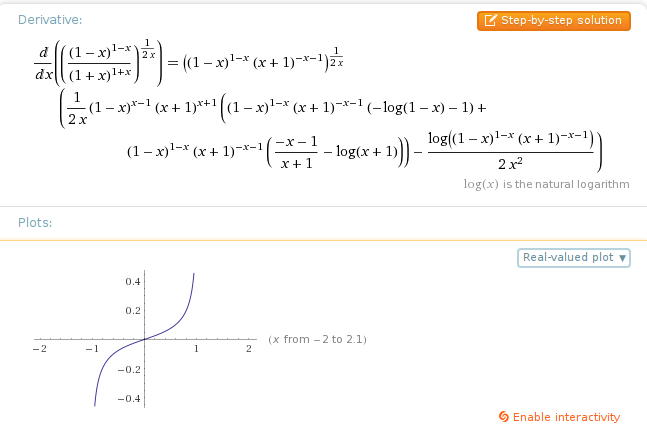
\includegraphics[width=\textwidth]{sheet-9/exercise-9-4}

  Yes, I could have used the derivative approach way earlier but I really wanted to try solving this just with algebraic manipulation.
\end{proof}

\end{document}
